\addcontentsline{toc}{section}{Introduction}

\section*{Introduction}

L'informatique décisionnelle, également connue sous le terme de Business Intelligence (BI), englobe les processus, les technologies et les outils utilisés pour collecter, stocker, analyser et présenter les données dans le but de soutenir la prise de décision et d'aider les entreprises à obtenir des informations exploitables. L'informatique décisionnelle implique la transformation des données brutes en informations significatives et en connaissances exploitables pour les décideurs. On va voir dans ce chaptire pourquoi on a decidé d'opter pour Delta Lake au lieu de ses contre-parts ainsi que les microservice et les microfrontends.

\section{Différence entre un data warehouse, un data lake, un datalakehouse et un delta lake}
\begin{enumerate}
    \item[$\bullet$] \textbf{Data Warehouse:} Un data warehouse est une base de données centralisée qui est spécifiquement conçue pour le reporting et l'analyse. Il stocke les données structurées provenant de différentes sources, les organise selon un modèle de données prédéfini et les optimise pour des requêtes analytiques. Les données dans un data warehouse sont généralement cohérentes, intégrées et historisées. Cependant, la construction et la maintenance d'un data warehouse peuvent être complexes et coûteuses.
    \item[$\bullet$] \textbf{Data Lake:} Un data lake est un référentiel de données centralisé qui stocke de grandes quantités de données brutes, structurées et non structurées. Contrairement au data warehouse, le data lake ne nécessite pas une modélisation préalable des données. Il offre une grande flexibilité et évolutivité pour stocker des données hétérogènes. Cependant, l'intégration et la qualité des données peuvent être des défis dans un data lake.
    \item[$\bullet$] \textbf{Datalakehouse:} Le datalakehouse est une architecture émergente qui combine les avantages du data warehouse et du data lake. Il permet de stocker et de traiter à la fois des données brutes et des données structurées dans un environnement centralisé. Cette approche hybride offre la flexibilité d'un data lake et la capacité d'analyse d'un data warehouse. Cependant, la mise en place d'un datalakehouse peut nécessiter des efforts supplémentaires pour garantir la qualité des données et l'efficacité des requêtes.
    \item[$\bullet$] \textbf{Delta Lake:} Delta Lake est une technologie qui s'intègre aux data lakes existants pour fournir des fonctionnalités supplémentaires, telles que la gestion des transactions ACID (Atomicité, Cohérence, Isolation, Durabilité), la gestion des mises à jour incrémentielles et la garantie de la cohérence des données. Delta Lake est construit sur Apache Parquet et Apache Arrow, ce qui permet d'accélérer les requêtes analytiques et d'améliorer les performances globales. Cependant, l'utilisation de Delta Lake peut nécessiter des compétences techniques supplémentaires et peut avoir un impact sur la complexité de l'architecture de données. 
\end{enumerate}

% \subsection{Avantages et inconvénients de chaque architecture}

\subsection{Data Warehouse}
\textbf{Avanatges:}
\begin{enumerate}
    \item Données cohérentes et intégrées
    \item Modélisation préalable des données pour une analyse optimisée
    \item Hautes performances pour les requêtes analytiques
\end{enumerate}

\textbf{Inconvénients:}
\begin{enumerate}
    \item Coût élevé de construction et de maintenance
    \item Complexité de la modélisation des données
    \item Limitations pour l'intégration de données non structurées
\end{enumerate}

\subsection{Data Lake}
\textbf{Avanatges:}
\begin{enumerate}
    \item Stockage économique de grandes quantités de données
    \item Flexibilité pour intégrer des données brutes et non structurées
    \item Capacité à traiter des données de différentes sources
\end{enumerate}

\textbf{Inconvénients:}
\begin{enumerate}
    \item Difficulté à maintenir la qualité des données et la gouvernance
    \item Besoin d'outils avancés pour l'analyse et le traitement des données
    \item Requiert des compétences techniques pour l'exploitation efficace des données
\end{enumerate}

\subsection{Datalakehouse}
\textbf{Avanatges:}
\begin{enumerate}
    \item Combinaison des avantages du data warehouse et du data lake
    \item Flexibilité pour stocker et analyser des données brutes et structurées
    \item Possibilité d'évoluer en fonction des besoins évolutifs
\end{enumerate}

\textbf{Inconvénients:}
\begin{enumerate}
    \item Nécessite des efforts supplémentaires pour la qualité des données
    \item Complexité accrue de l'architecture de données
    \item Besoin de compétences techniques pour la mise en place et la gestion
\end{enumerate}

\subsection{Delta Lake (Datalakehouse)}
\textbf{Avanatges:}
\begin{enumerate}
    \item Gestion des transactions ACID pour une cohérence des données
    \item Prise en charge des mises à jour incrémentielles et du traitement des flux de données
    \item Hautes performances pour les requêtes analytiques
\end{enumerate}

\textbf{Inconvénients:}
\begin{enumerate}
    \item Nécessite des compétences techniques spécifiques
    \item Impact sur la complexité de l'architecture de données existante
    \item Peut nécessiter des adaptations pour une intégration transparente avec les outils existants
\end{enumerate}

\begin{figure}[H]
\centering
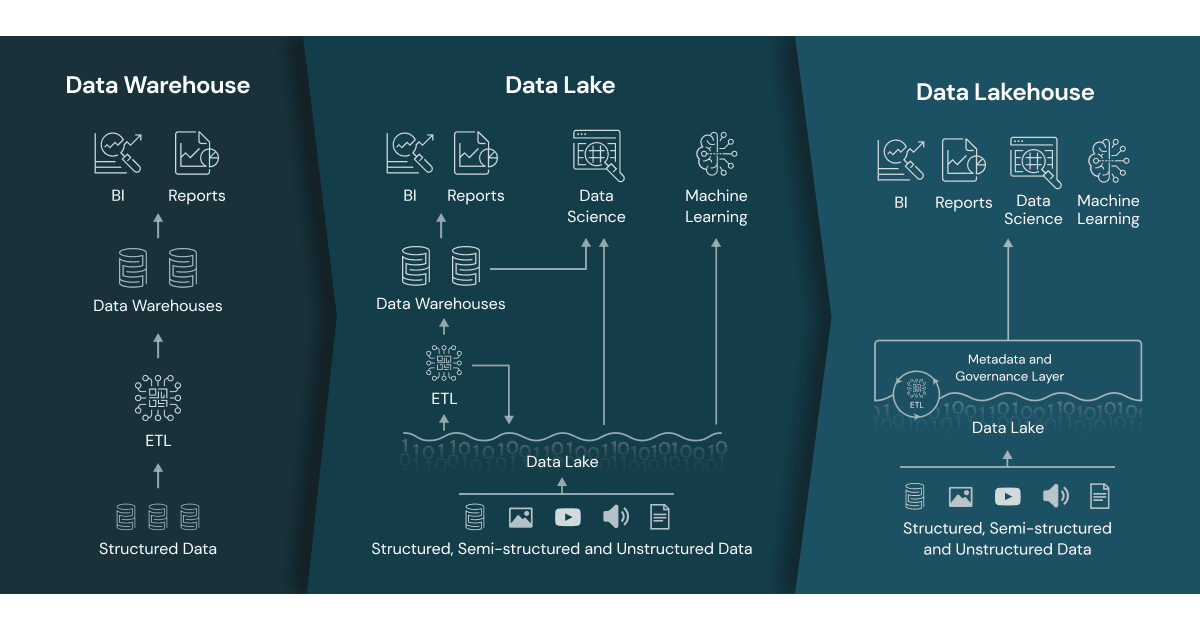
\includegraphics[width=\linewidth]{images/data-warehouse-data-lake-datalakehouse.png}
\caption{Data Warehouse vs Data Lake vs Data Lakehouse}\label{fig:data-warehouse-data-lake-datalakehouse}
\end{figure}

\section{Différence entre une architecture microservices et une architecture monolithique}
\begin{enumerate}
    \item[$\bullet$] \textbf{Monolithe:} un monolithe est une application qui est conçue comme une entité unique et indivisible. Toutes les fonctionnalités de l'application sont regroupées dans un seul code base, partageant les mêmes ressources, bases de données et déploiements. Dans une architecture monolithique, il n'y a pas de découpage clair des fonctionnalités en services indépendants. Toute modification ou évolution de l'application nécessite des changements au niveau global.
    \item[$\bullet$] \textbf{Microservice:} Un microservice est une approche architecturale dans laquelle une application est construite comme un ensemble de services indépendants et autonomes, chacun se concentrant sur une fonction spécifique de l'application. Chaque microservice est développé, déployé et géré de manière indépendante, ce qui permet une évolutivité, une flexibilité et une maintenance plus faciles. Les microservices communiquent entre eux via des interfaces bien définies, généralement basées sur des API REST ou des messages.
\end{enumerate}

\subsection{Avantages et Inconvénients de l'architecture monolithique}
\textbf{Avanatges:}
\begin{enumerate}
    \item \textbf{Simplicité de développement initial :} L'approche monolithique permet de développer rapidement une application en regroupant toutes les fonctionnalités dans un seul code base. Cela facilite la gestion des dépendances et la coordination des différentes parties de l'application.
    \item \textbf{Moins de complexité opérationnelle :} Avec une architecture monolithique, il y a moins de composants et de services à gérer, ce qui simplifie les opérations de déploiement, de surveillance et de gestion. Tout est regroupé au sein d'un seul déploiement, ce qui peut être plus facile à gérer pour les équipes opérationnelles.
    \item \textbf{Communications internes plus rapides :} Dans une architecture monolithique, les communications entre les différentes parties de l'application sont plus rapides car elles se font généralement via des appels de méthode internes. Cela peut être bénéfique en termes de performances et de latence réduite.
\end{enumerate}

\textbf{Inconvénients:}
\begin{enumerate}
    \item \textbf{Difficulté à faire évoluer et à maintenir:} Avec une architecture monolithique, les évolutions et les mises à jour peuvent être plus complexes, car chaque changement doit être effectué sur l'ensemble de l'application. Cela peut rendre le processus de développement plus lent et entraîner des risques d'erreurs lors des déploiements.
    \item \textbf{Rigidité technologique:} Une architecture monolithique peut entraîner une rigidité technologique, car toutes les parties de l'application doivent utiliser les mêmes technologies et langages de programmation. Cela peut limiter les possibilités d'adopter de nouvelles technologies ou de faire évoluer des parties spécifiques de l'application de manière indépendante.
    \item \textbf{Difficulté à isoler les problèmes:} En cas de problème ou de bug, il peut être plus difficile de les isoler et de les résoudre dans une architecture monolithique. Étant donné que toutes les fonctionnalités sont regroupées dans un seul code base, il peut être complexe de localiser l'origine exacte du problème.
    \item \textbf{Moins de flexibilité en termes d'évolutivité:} L'architecture monolithique peut poser des défis en termes d'évolutivité. Si une partie de l'application nécessite plus de ressources pour gérer une charge élevée, il peut être difficile d'ajuster cette partie spécifique sans augmenter les ressources globales de l'application.
\end{enumerate}

\subsection{Avantages et Inconvénients de l'architecture microservices}
\textbf{Avanatges:}
\begin{enumerate}
    \item \textbf{Scalabilité et évolutivité:} Les microservices permettent de découper l'application en plusieurs services autonomes et indépendants, ce qui facilite la scalabilité horizontale. Chaque microservice peut être déployé, mis à l'échelle et mis à jour indépendamment, ce qui permet de gérer efficacement les variations de charge et de garantir une évolutivité facile en fonction des besoins de l'entreprise.
    \item \textbf{Flexibilité technologique:} Les microservices offrent la possibilité d'utiliser différentes technologies et langages de programmation pour chaque service. Dans notre cas, l'utilisation de Spring Boot nous permet de profiter de son écosystème riche et de ses fonctionnalités avancées pour le développement rapide d'applications. Cela permet également d'adopter des technologies spécifiques en fonction des besoins de chaque microservice, favorisant ainsi la flexibilité technologique.
    \item \textbf{Indépendance et autonomie:} Chaque microservice est conçu pour fonctionner de manière autonome, ce qui permet une meilleure isolation des fonctionnalités et des responsabilités. Cela facilite la maintenance, le test et le déploiement des services de manière indépendante, réduisant ainsi les risques d'impact sur l'ensemble du système en cas de modifications ou de problèmes.
    \item \textbf{Développement et déploiement rapides:} Les microservices permettent une approche de développement agile en favorisant des cycles de développement plus courts. Les équipes peuvent se concentrer sur des fonctionnalités spécifiques et les développer de manière indépendante, ce qui accélère le développement global du système. De plus, les microservices peuvent être déployés de manière continue grâce à l'utilisation de techniques de déploiement automatisées, facilitant ainsi les mises à jour fréquentes et rapides.
    \item \textbf{Facilité de maintenance et de débogage:} En raison de leur nature modulaire, les microservices facilitent la maintenance et le débogage du système. En cas de problème ou d'erreur, il est plus facile d'identifier le service spécifique concerné et de résoudre le problème sans impacter l'ensemble du système.
\end{enumerate}

\textbf{Inconvénients:}
\begin{enumerate}
    \item \textbf{Complexité de la gestion des communications:} Les microservices impliquent une communication entre différents services, généralement via des API REST ou des messages. La gestion de ces communications peut devenir complexe, en particulier lorsque de nombreux services sont impliqués. Des problèmes tels que la latence, la cohérence des données et la gestion des erreurs peuvent se poser.
    \item \textbf{Surcharge de développement initial:} Le développement de microservices nécessite un effort supplémentaire pour découper correctement les fonctionnalités, définir les interfaces et mettre en place une infrastructure appropriée pour le déploiement et la communication des services. Cela peut augmenter la charge de travail initiale et nécessiter des compétences spécifiques en matière d'architecture distribuée.
    \item \textbf{Gestion de la cohérence des données:} Avec des microservices, chaque service peut avoir sa propre base de données ou son propre stockage de données. Cela peut rendre la gestion de la cohérence des données plus complexe, en particulier lorsqu'il y a des mises à jour simultanées impliquant plusieurs services. Des techniques telles que les transactions distribuées ou les événements asynchrones peuvent être nécessaires pour maintenir la cohérence des données.
    \item \textbf{Déploiement et gestion de plusieurs services:} Avec les microservices, il y a un nombre accru de services à déployer, gérer et surveiller. Cela peut nécessiter des compétences supplémentaires en matière d'automatisation des déploiements, de gestion des conteneurs ou de gestion des clusters. Le suivi des performances et du comportement de chaque service peut également devenir plus complexe.
    \item \textbf{Coût de l'infrastructure:} Les microservices peuvent nécessiter une infrastructure plus complexe et des ressources supplémentaires pour fonctionner efficacement. Chaque service doit être déployé et exécuté indépendamment, ce qui peut entraîner une augmentation des coûts liés aux ressources informatiques et à la gestion de l'infrastructure.
\end{enumerate}

\begin{figure}[H]
\centering
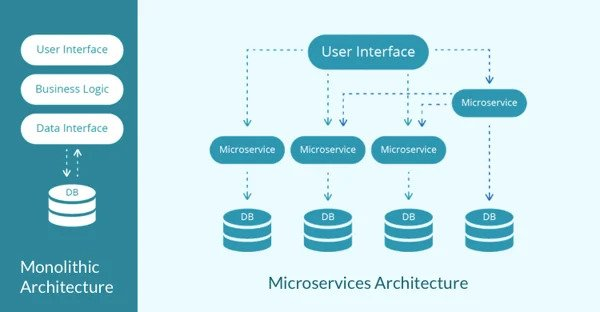
\includegraphics[width=0.6\linewidth]{images/monolithicvsmicroservice.jpg}
\caption{Architecture monolithique vs microservice}\label{fig:monolithevsmicroservice}
\end{figure}

\section{Différence entre une architecture microfrontends et une architecture monolithique frontend}
\begin{enumerate}
    \item[$\bullet$] \textbf{Monolithe frontend:} Un frontend monolithique est une approche architecturale où l'application frontend est développée comme une seule entité, généralement en utilisant un framework spécifique tel qu'AngularJS. Toutes les fonctionnalités, les vues et les logiques de l'interface utilisateur sont regroupées dans un seul code base.
    \item[$\bullet$] \textbf{Microfrontends:} Les microfrontends sont une approche architecturale où une application frontend est divisée en plusieurs micro-applications indépendantes, chacune étant responsable d'une partie spécifique de l'interface utilisateur. Chaque micro-application peut être développée, déployée et évoluée de manière autonome, utilisant différents frameworks, langages et technologies.
\end{enumerate}

\subsection{Avantages et Inconvénients du monolithe frontend}
\textbf{Avanatges:}
\begin{enumerate}
    \item \textbf{Simplicité de développement initial:} L'architecture monolithique avec AngularJS offre une approche simple pour le développement initial de l'application frontend. Toutes les fonctionnalités sont regroupées dans un seul code base, ce qui facilite la coordination et la gestion du développement.
    \item \textbf{Facilité de communication entre les composants:} Dans une architecture monolithique, les composants AngularJS peuvent communiquer entre eux facilement via le système de directives et de services d'AngularJS. Cela permet une communication rapide et efficace entre les différentes parties de l'application. 
    \item \textbf{Interopérabilité des fonctionnalités:} Étant donné que toutes les fonctionnalités sont développées en utilisant AngularJS, il est plus facile de partager des fonctionnalités et des modules entre les différentes parties de l'application. Cela favorise la réutilisation du code et simplifie la maintenance.
\end{enumerate}

\textbf{Inconvénients:}
\begin{enumerate}
    \item \textbf{Difficulté à maintenir et à faire évoluer:} À mesure que l'application frontend devient plus complexe, la maintenance et l'évolution de l'architecture monolithique avec AngularJS peuvent devenir difficiles. Les modifications apportées à une partie de l'application peuvent avoir des répercussions sur l'ensemble du code base, ce qui rend le processus de développement plus lent et risqué.
    \item \textbf{Limitations de performance:} Dans une architecture monolithique, toutes les fonctionnalités sont chargées en même temps, ce qui peut entraîner des problèmes de performance si l'application devient volumineuse. Les temps de chargement peuvent être plus longs et l'application peut être moins réactive pour l'utilisateur.
    \item \textbf{Flexibilité limitée:} L'architecture monolithique avec AngularJS peut limiter la flexibilité technologique. Étant donné que toutes les parties de l'application sont développées en utilisant AngularJS, il peut être difficile d'introduire de nouvelles technologies ou de faire évoluer certaines parties spécifiques de l'application de manière indépendante.
\end{enumerate}

\subsection{Avantages et Inconvénients de l'architecture microfrontends}
\textbf{Avanatges:}
\begin{enumerate}
    \item \textbf{Indépendance des équipes de développement:} Chaque micro-application peut être développée par une équipe distincte, ce qui favorise une plus grande autonomie et une meilleure collaboration entre les équipes de développement. Chaque équipe peut choisir les technologies qui conviennent le mieux à ses besoins.
    \item \textbf{Évolutivité et facilité de maintenance:} L'architecture microfrontends permet de faire évoluer et de maintenir les différentes parties de l'application de manière indépendante. Les modifications apportées à une micro-application n'ont pas d'impact sur les autres, ce qui facilite la maintenance et permet de déployer rapidement de nouvelles fonctionnalités.
    \item \textbf{Flexibilité technologique:} Chaque micro-application peut utiliser la technologie, le framework ou le langage de programmation qui convient le mieux à son domaine spécifique. Cela permet d'introduire de nouvelles technologies et d'exploiter les avantages des derniers développements dans le domaine de l'ingénierie logicielle.
\end{enumerate}

\textbf{Inconvénients:}
\begin{enumerate}
    \item \textbf{Complexité accrue:} L'architecture microfrontends introduit une certaine complexité dans le développement et le déploiement de l'application. La gestion des interactions et de la communication entre les différentes micro-applications peut nécessiter une planification et une coordination supplémentaires.
    \item \textbf{Coût de développement initial:} Le développement d'une architecture microfrontends peut nécessiter un investissement initial plus important en termes de ressources et de temps. Le développement de plusieurs micro-applications distinctes et la mise en place de l'infrastructure nécessaire peuvent être plus coûteux que le développement d'une application monolithique.
    \item \textbf{Surcharge réseau:} L'utilisation d'une architecture microfrontends peut entraîner une surcharge réseau plus importante, car chaque micro-application nécessite des requêtes et des chargements de ressources distincts. Cela peut avoir un impact sur les performances de l'application et nécessiter une gestion efficace du réseau.
\end{enumerate}

\begin{figure}[H]
\centering
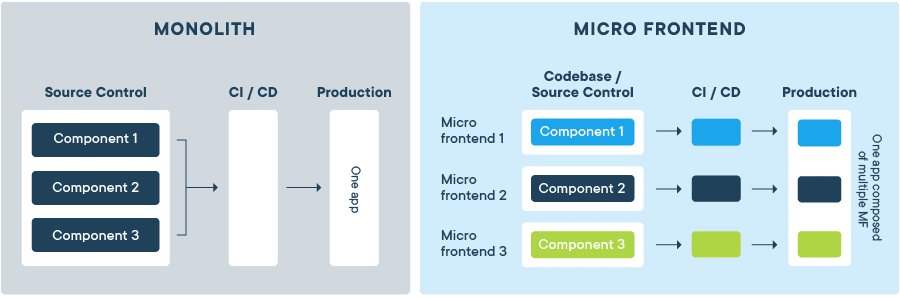
\includegraphics[width=\linewidth]{images/micro-frontend-vs-monolith-frontend.png}
\caption{Architecture monolithique frontend vs microfrontends}\label{fig:monolithfrontendvsmicrofrontends}
\end{figure}

\section{Cheminement de la solution}
\subsection{Partie Data}
Dans le cadre de notre solution, nous avons opté de remplacer l'exporter worker existant et les bases de données MariaDB par de remplacer l'exporter worker existant et les bases de données MariaDB par l'utilisation d'une architecture de type datalakehouse. Une datalakehouse est une approche hybride qui combine les avantages d'un data warehouse et d'un data lake, offrant ainsi une solution plus flexible et évolutive pour la gestion des données.

\subsection{Partie Backend}
Pour la mise en œuvre des microservices, nous avons opté d'utiliser Spring Boot, un framework Java populaire pour le développement d'applications. En utilisant Spring Boot, nous pouvons créer des microservices autonomes, indépendants les uns des autres, qui peuvent être développés, déployés et scalés individuellement. Spring Boot fournit également des fonctionnalités telles que la gestion de la persistance des données, la sécurité et la création d'API REST, ce qui facilite le développement des microservices.

\begin{figure}[H]
\centering
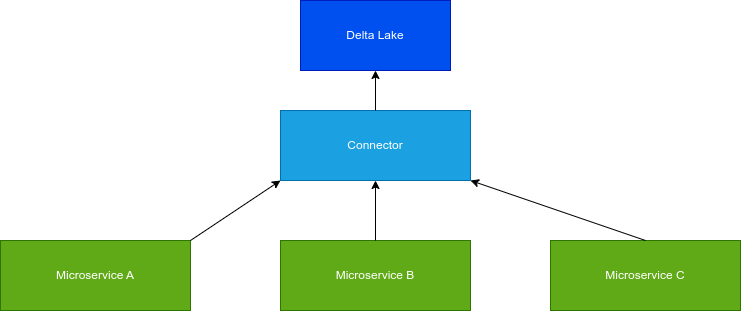
\includegraphics[width=\linewidth]{images/delta-lake-microservices.png}
\caption{Delta lake connectés à des microservices}\label{fig:schema-delta}
\end{figure}

\subsection{Partie Frontend}
Pour la mise en œuvre des microfrontends, Nous avons choisie d'utiliser principalement React pour les microfrontends, l'équipe de développement peut bénéficier de l'écosystème riche et mature de React, ainsi que de sa popularité croissante dans l'industrie du développement frontend. Cependant, il est également mentionné qu'Angular peut être utilisé ultérieurement si nécessaire, offrant ainsi une flexibilité supplémentaire dans le choix des technologies.

\begin{figure}[H]
\centering
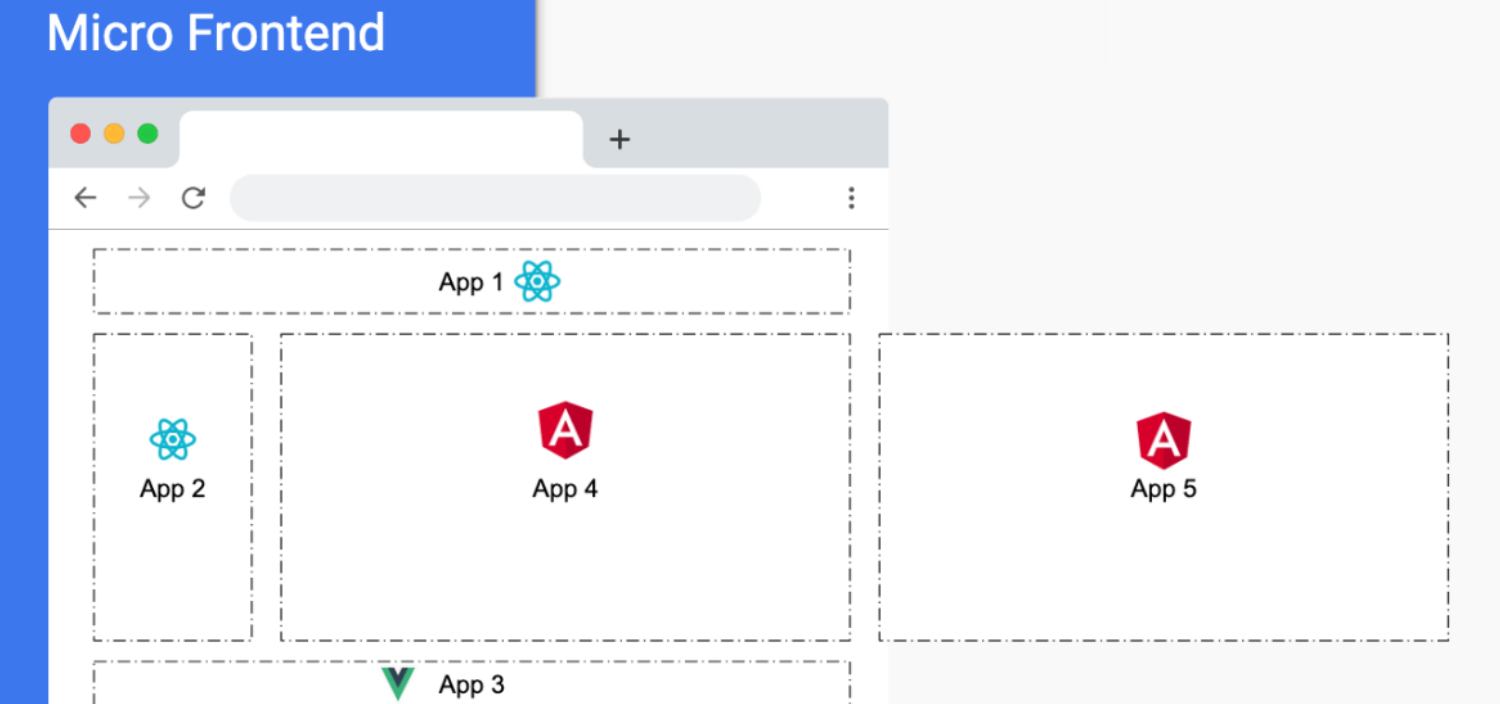
\includegraphics[width=\linewidth]{images/microfrontends.png}
\caption{Schéma des microfrontends}\label{fig:schema-microfrontends}
\end{figure}

\section*{Conclusion}
\addcontentsline{toc}{section}{Conclusion}
Lors de l'évaluation des différentes architectures de données pour Izicap, il est important de comprendre les besoins spécifiques liés à la gestion des fichiers bancaires, des reçus de transactions et des opérations d'agrégation.

Un data warehouse aurait pu être une option envisageable, offrant des structures de données organisées et optimisées pour les requêtes analytiques. Cependant, le principal inconvénient d'un data warehouse réside dans sa nature statique, qui nécessite une modélisation préalable des données et une transformation rigide avant leur chargement. Cela peut poser des défis lors de l'intégration de nouveaux types de fichiers ou de l'évolution des besoins en matière d'agrégation.

D'autre part, un data lake présente des avantages en termes de stockage économique et de flexibilité pour intégrer des données brutes et non structurées. Cependant, il peut être plus complexe de maintenir la qualité des données et la gouvernance, et des compétences techniques spécifiques sont nécessaires pour exploiter efficacement les données du data lake.

Donc, Delta Lake a été privilégié en raison de sa capacité à répondre aux besoins spécifiques d'Izicap en matière de gestion des fichiers bancaires, des reçus de transactions et des opérations d'agrégation. Il offre la flexibilité et la performance nécessaires tout en maintenant l'intégrité des données, ce qui en fait un choix solide pour l'architecture de données de l'entreprise.

En adoptant une approche basée sur les microservices, Izicap peut améliorer la flexibilité, la scalabilité et la maintenance de son application frontend. Cela permettra à l'entreprise de mieux répondre aux besoins changeants de ses utilisateurs, de faciliter la collaboration entre les équipes de développement et d'adopter des technologies innovantes pour offrir une expérience utilisateur optimale.

Les microfrontends offrent plusieurs avantages pour Izicap. Tout d'abord, la modularité inhérente aux microfrontends permet de développer, déployer et maintenir différentes parties de l'interface utilisateur de manière indépendante. Cela favorise la collaboration entre les équipes de développement et permet d'évoluer rapidement et efficacement. Chaque micro-application peut être développée en utilisant le framework et les technologies les plus adaptés à ses besoins spécifiques, ce qui offre une flexibilité technologique essentielle pour Izicap.

En revanche, l'approche monolithique présente des limitations en termes de scalabilité et de flexibilité technologique. Les modifications apportées à une partie de l'application peuvent avoir un impact sur l'ensemble du système, ce qui rend les évolutions plus complexes et risquées. De plus, l'introduction de nouvelles technologies ou frameworks peut être difficile dans une architecture monolithique, ce qui limite les possibilités d'innovation et de modernisation.

